\usetikzlibrary {arrows.meta} 
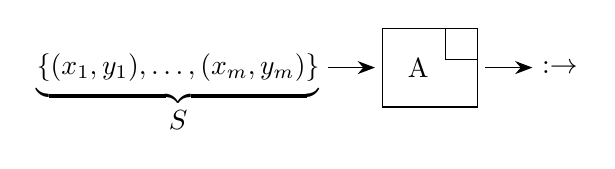
\begin{tikzpicture}

    \node at (0.4,1.5) {$\{(x_1,y_1),\dots,(x_m,y_m)\}$};
    \node at (0.4,1.15) {$\underbrace{\phantom{\{(x_1,y_1),\dots,(x_m,y_m)\}}}_{\displaystyle S}$};
    \draw[-{Stealth[length=2.2mm]}] (2.3,1.5) -- (2.9,1.5);
    \draw (3,2) rectangle (4.2,1);
    \node at (3.45,1.5) {A};
    \draw (3.8,2) rectangle (4.2,1.6) node[pos=.5] {$\loss$};
    \draw[-{Stealth[length=2.2mm]}] (4.3,1.5) -- (4.9,1.5)
        node [right] {$\pred: \X \rightarrow \Y$};

\end{tikzpicture}